% 
\documentclass[cic,tc]{iiufrgs}

% Use unicode
\usepackage[utf8]{inputenc}   % pacote para acentuação

% Necessário para incluir figuras
\usepackage{graphicx}         % pacote para importar figuras

\usepackage{times}            % pacote para usar fonte Adobe Times
% \usepackage{palatino}
% \usepackage{mathptmx}       % p/ usar fonte Adobe Times nas fórmulas

\usepackage[alf,abnt-emphasize=bf]{abntex2cite}	% pacote para usar citações abnt

\usepackage{array}
% 
% Informações gerais
% 
\title{Implementação e Avaliação de um Mecanismo de Detecção de Ameaças em uma Ferramenta Smart Grid}

\author{Eitelvein}{Luiza dos Santos}

\advisor[Prof.~Dr.]{Schaeffer-Filho}{Alberto Egon}

% a data deve ser a da defesa; se nao especificada, são gerados
% mes e ano correntes
% \date{dezembro}{2015}

 \location{Porto Alegre}{RS}

% itens individuais da nominata podem ser redefinidos com os comandos
% abaixo:
% \renewcommand{\nominataReit}{Prof\textsuperscript{a}.~Wrana Maria Panizzi}
% \renewcommand{\nominataReitname}{Reitora}
% \renewcommand{\nominataPRE}{Prof.~Jos{\'e} Carlos Ferraz Hennemann}
% \renewcommand{\nominataPREname}{Pr{\'o}-Reitor de Ensino}
% \renewcommand{\nominataPRAPG}{Prof\textsuperscript{a}.~Joc{\'e}lia Grazia}
% \renewcommand{\nominataPRAPGname}{Pr{\'o}-Reitora Adjunta de P{\'o}s-Gradua{\c{c}}{\~a}o}
% \renewcommand{\nominataDir}{Prof.~Philippe Olivier Alexandre Navaux}
% \renewcommand{\nominataDirname}{Diretor do Instituto de Inform{\'a}tica}
% \renewcommand{\nominataCoord}{Prof.~Carlos Alberto Heuser}
% \renewcommand{\nominataCoordname}{Coordenador do PPGC}
% \renewcommand{\nominataBibchefe}{Beatriz Regina Bastos Haro}
% \renewcommand{\nominataBibchefename}{Bibliotec{\'a}ria-chefe do Instituto de Inform{\'a}tica}
% \renewcommand{\nominataChefeINA}{Prof.~Jos{\'e} Valdeni de Lima}
% \renewcommand{\nominataChefeINAname}{Chefe do \deptINA}
% \renewcommand{\nominataChefeINT}{Prof.~Leila Ribeiro}
% \renewcommand{\nominataChefeINTname}{Chefe do \deptINT}

% 
% palavras-chave
% iniciar todas com letras minúsculas, exceto no caso de abreviaturas
% 
\keyword{smart grid}


%\settowidth{\seclen}{1.10~}

% 
% inicio do documento
% 
\begin{document}

% folha de rosto
% às vezes é necessário redefinir algum comando logo antes de produzir
% a folha de rosto:
% \renewcommand{\coordname}{Coordenadora do Curso}
\maketitle

% dedicatoria
% \clearpage
% \begin{flushright}
%     \mbox{}\vfill
%     {\sffamily\itshape
%       ``If I have seen farther than others,\\
%       it is because I stood on the shoulders of giants.''\\}
%     --- \textsc{Sir~Isaac Newton}
% \end{flushright}

% agradecimentos
%\chapter*{Agradecimentos}
%Agradeço ao \LaTeX\ por não ter vírus de macro\ldots



% resumo na língua do documento
\begin{abstract}
    Resumo em português.
\end{abstract}

% resumo na outra língua
% como parametros devem ser passados o titulo e as palavras-chave
% na outra língua, separadas por vírgulas
\begin{englishabstract}{Implementation and Evaluation of a Threat Detection Mechanism in a Smart Grid Tool}{Smart Grid}
    Abstract in English.
\end{englishabstract}

% lista de figuras
% \listoffigures

% lista de tabelas
% \listoftables

% lista de abreviaturas e siglas
% o parametro deve ser a abreviatura mais longa
\begin{listofabbrv}{SCADA}
    \item[SCI]   Sistema de Controle Industrial
    \item[CLP]   Controlador Lógico Programável
    \item[TIC]   Tecnologia da Informação e Comunicação
    \item[HMI]   Interface Homem-Máquina
    \item[DEI]   Dispositivos Eletrônicos Inteligente
    \item[UTR]   Unidade Terminal Remota
    \item[SCADA] Supervisory Control and Data Acquisition
    
\end{listofabbrv}

% idem para a lista de símbolos
% \begin{listofsymbols}{$\alpha\beta\pi\omega$}
%     \item[$\sum{\frac{a}{b}}$] Somatório do produtório
%     \item[$\alpha\beta\pi\omega$] Fator de inconstância do resultado
% \end{listofsymbols}

% sumario
\tableofcontents

\chapter{Introdução}
\section{Motivação}
\section{Objetivos}
\section{Contribuição}
\section{Estrutura do Trabalho}
\chapter{Fundamentação Teórica}
\section{Smart Grids}
Smart Grids combinam redes de energia elétrica com estruturas de comunicação, baseadas em Tecnologia de Informação e Comunicação (TIC), que provêm um meio de troca de dados entre os componentes envolvidos no processo de produção, distribuição e consumo de energia. Como suas principais características, podem ser mencionados o fluxo bidirecional de energia elétrica entre produtores e consumidores e a incorporação de uma infraestrutura de comunicação, também bidirecional, que provê uma maior capacidade de automação à rede \cite{2013survey}. Através de recursos e técnicas como monitoramento em tempo real, automação e controle de dispositivos, autoavaliação e autorecuperação, integração com de fontes de energia alternativas e mecanismos de segurança física e cibernética, Smart Grids imbuem a rede elétrica com maior confiabilidade, eficiência e segurança \cite{li2012securing}.

\subsection{Arquitetura}

A produção de energia em um smart grid está distribuída em diversas fontes, que incluem usinas fixas e móveis e microprodutores. A energia elétrica é transportada das usinas de geração até as subestações de transmissão através de cabos de alta tensão, e então é transmitida, assim como a energia de outras fontes diversas, até as subestações de distribuição através de linhas de tensão variada. A partir das subestações de distribuição, finalmente, a energia é distribuída para consumo \cite{harb2013communication}.

Cada consumidor de um smart grid, em conjunto com um medidor inteligente e disjuntores de controle forma uma rede residencial. Redes residenciais, Dispositivos Eletrônicos Inteligentes (DEIs) e Unidades Terminais Remotas (UTRs) são agrupados em redes de comunidades que, por sua vez, são conectadas a produtores de energia e outros elementos do smart grid em uma área geográfica por uma rede regional \cite{li2012securing}. Controle e monitoramento da rede em cada região são realizados por centros de controle regionais que implementam sistemas de Controle de Supervisão e Aquisição de Dados – \textit{Supervisory Control and Data Acquisition (SCADA)}. Sensores inteligentes instalados ao longo de toda a extensão da rede coletam, em tempo real, informações detalhadas sobre o consumo de energia e os transmitem para centrais de dados, formando uma Infraestrutura de Monitoramento Avançada (IMA) \cite{2013survey}. A figura \ref{fig:sgarchitecture} ilustra a arquitetura genérica da infraestrutura de um smart grid.

\begin{figure}[h]
   \caption{Arquitetura de um smart grid}
   \begin{center}
       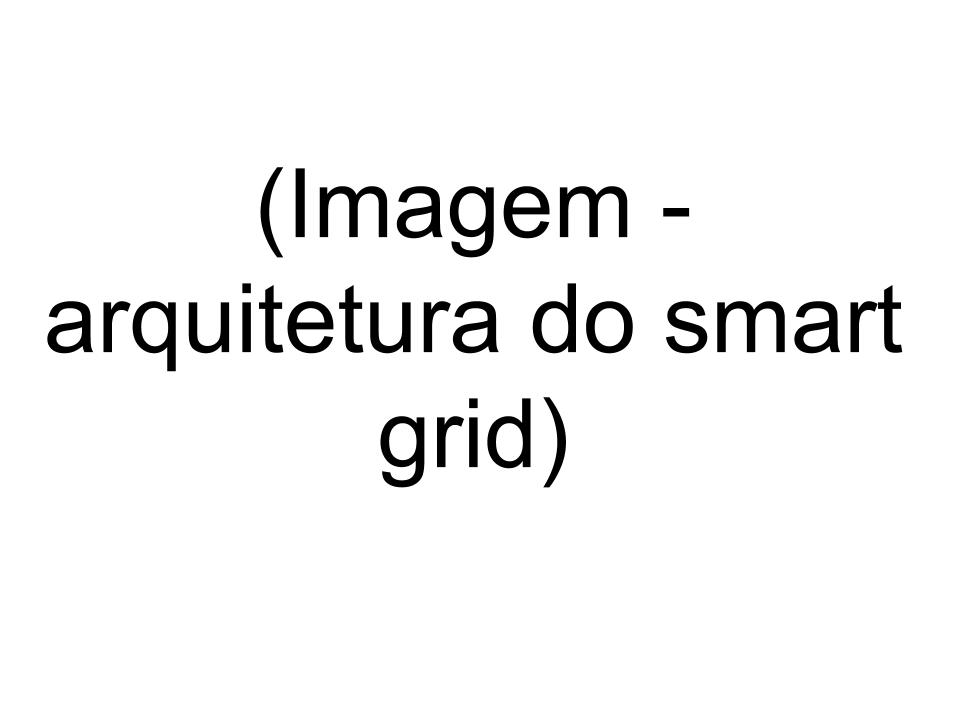
\includegraphics[width=12em]{tmp_img}
   \end{center}
   \legend{Fonte: Autor}
   \label{fig:sgarchitecture}
\end{figure}

\subsection{Motivação}

A  infraestrutura de comunicação dos Smart Grids incorpora uma grande diversidade de benefícios ao sistema de produção, distribuição e consumo de energia. Dados coletados pela IMA podem ser utilizados para melhorar a eficiência e o desempenho da distribuição de energia, identificando picos de consumo e pontos de desperdício na rede, além de fornecer aos usuários informações detalhadas sobre seu consumo de energia, levando-os a um consumo mais eficiente. Uma maior automação da rede de distribuição leva à diminuição dos custos operacionais, pois seu funcionamento torna-se mais independente da mão de obra envolvida, que, por sua vez, pode executar suas tarefas com mais eficiência. A capacidade de comunicação entre diversas entidades e o fluxo bidirecional de energia possibilitam uma utilização cada vez maior de recursos de energia distribuídos, incentivando o surgimento de fontes de geração de energia renovável, como solar e eólica. Entidades consumidoras podem também ser produtoras de energia, permitindo que microprodutores forneçam energia à rede simultaneamente a grandes produtores \cite{2013survey}.

A capacidade de autoavaliação e autoajuste em redes elétricas e outras infraestruturas críticas, como sistemas de transporte e financeiros, é de imensa importância. Devido à modernização das tecnologias utilizadas, essas infraestruturas têm seus sistemas cada vez mais interconectados, aumentando o risco de falhas em cascata de grandes proporções. A demanda crescente por uma distribuição de energia mais eficiente e confiável traz a necessidade de aperfeiçoar métodos e ferramentas que forneçam às redes elétricas a capacidade de se autoregular e sofrer o mínimo impacto possível na ocorrência de sobrecarga, mal funcionamento ou ataques maliciosos \cite{massoud2005toward}.

\subsection{Ameaças}

A introdução de uma estrutura de comunicação autônoma e amplamente distribuída que ampara todo o funcionamento da rede elétrica expõe todo o sistema à possibilidade de ataques cibernéticos. A infraestrutura de comunicação, por ser desenvolvida sobre TIC, é inerentemente vulnerável a diversos tipos de ataque, que podem ser utilizados para manipular dados ou obstruir o funcionamento do sistema \cite{pin2012smart}. Medidores inteligentes também são potencialmente inseguros, estando vulneráveis a ataques de negação de serviço, roubo de informações de usuários e manipulação de dados \cite{ashford2011smartmeter}.

A evolução dos ataques cibernéticos e o risco que representam para infraestruturas críticas podem ser observados em fenômenos como o Stuxnet, um \textit{malware} desenvolvido para atacar controladores de sistemas industriais. O Stuxnet insere código ilegítimo na execução do controlador, que passa a ser executado em detrimento do código original, sem ser detectado, podendo levar à interrupção do serviço e danificar componentes do sistema atingido \cite{langner2011stuxnet}.

Uma taxonomia dos tipos de ataques cibernéticos em estruturas de comunicação de smart grids é apresentada em \cite{li2012securing}. Os autores descrevem quatro tipos de ataques, como apresentados na tabela \ref{tbl:attacktypes}: ataques a dispositivos, ataques de dados, ataques de privacidade e ataques de disponibilidade de rede.

\subsubsection{Ataques a dispositivos}
Ataques a dispositivos têm como finalidade obter controle sobre um elemento do smart grid e utilizá-lo para um objetivo malicioso. De modo geral, servem a dois propósitos: fornecer os meios para um ataque de dados ou de disponibilidade ou, caso o dispositivo afetado possua funções de controle críticas, causar danos físicos ao sistema.

\subsubsection{Ataques de dados}
Ataques de dados configuram a tentativa de manipular os dados presentes na rede. Os dados manipulados podem ser informações de usuários ou sinais dos dispositivos de controle do smart grid. Seus usos variam de alterar dados de um usuário, para reduzir o valor da energia consumida, a eliminar sinais enviados por dispositivos de controle, para impedir o monitoramento e diagnóstico dos elementos da rede, o que pode levar a interrupção do funcionamento do sistema.

\subsubsection{Ataques de privacidade}
Ataques de privacidade têm o objetivo de obter informações privativas dos usuários. No caso dos smart grids, essas informações são os dados sobre o consumo de energia elétrica dos usuários, transmitidos pela rede de comunicação. Essas informações podem ser utilizadas para mapear dados privativos sobre a rotina dos usuários, que podem ser utilizados para fins maliciosos.

\subsubsection{Ataques de disponibilidade}
Ataques de disponibilidade de rede, ou ataques de negação de serviço, causam lentidão no tráfego de dados do smart grid através da sobrecarga da rede de comunicação e recursos computacionais. A velocidade da troca de dados é crítica para o funcionamento de um smart grid, e lentidão ou indisponibilidade do tráfego da rede podem causar prejuízos sérios aos seus usuários.

\begin{table}[h]
   \caption{Taxonomia dos tipos de ataques cibernéticos em smart grids}
   \centering
       \begin{tabular}{p{4cm}|p{8cm}}
         \hline
         Nome  &  Descrição\\
         \hline
         \hline
         Ataques a dispositivos & Têm como objetivo comprometer (controlar) um dispositivo da rede. Frequentemente, é o passo inicial de um ataque sofisticado.\\
         \hline
		Ataques de dados & Tentam inserir, alterar ou deletar dados no tráfego da rede para induzir o smart grid a tomar decisões erradas.\\
 \hline
		Ataques de privacidade & Têm como objetivo obter/inferir informações privadas do usuário analizando dados sobre a utilização de energia elétrica.\\
 \hline
		Ataques de disponibilidade de rede & Visam esgotar ou sobrecarregar os recursos de comunicação e computacionais do smart grid para causar atraso ou falha de comunicação. \\
         \hline
       \end{tabular}
   \legend{Fonte: \cite{li2012securing}}
\label{tbl:attacktypes}
\end{table}

\section{Mecanismos de Detecção}
\section{Ferramentas de Simulação}

\subsection{VirtuaPlant}
VirtuaPlant \cite{virtuaplantwebsite} é um simulador de Sistemas de Controle Industriais (SCI). Possui uma interface gráfica chamada World View que simula o efeito das ações do sistema de controle sobre um recurso virtual utilizando protocolo Modbus. O recurso é representado por uma fábrica que enche garrafas.
	
O Controlador Lógico Programável (CLP) é implementado sobre a biblioteca pymodbus, que roda em uma thread separada no componente World View e compartilha seu contexto, que contém registradores, entradas e valores, com as funções do World View para simular recursos sendo conectados ao controlador.

A Interface Homem-Máquina (HMI) utiliza GTK3 e executa o cliente pymodbus em uma thread separada, que conecta com o servidor através de TCP/IP, obtendo leituras constantes dos valores do servidor, isto é, do CLP.

A ferramenta VirtuaPlant fornece uma variedade de scripts de ataque ao CLP. Entretanto, não permite a definição de novos dispositivos, não sendo possível a definição de novas topologias. Também não possibilita a modelagem de elementos da infraestrutura de comunicação, já que a simulação engloba apenas a leitura e escrita dos valores do controlador PLC.

\subsection{Mosaik}
O Mosaik \cite{mosaikwebsite} permite usar diversos simuladores existentes em um contexto comum para realizar uma simulação coordenada de um cenário, que representa um conjunto de componentes de smart grid. Oferece uma API para os simuladores se comunicarem com ele e possui handlers para cada tipo de processo dos simuladores.
	
A ferramenta permite a modelagem de diferentes cenários envolvendo esses simuladores, possibilitando a criação de novos objetos e definição de novas topologias. A biblioteca SimPy é utilizada para a simulação coordenada de cenários, e a execução da simulação é feita executando passos em cada simulador ao longo do tempo. Cada simulador executa o seu próprio processo e loop de eventos, enquanto o Mosaik sincroniza esses processos e gerencia a troca de dados entre eles. Através da combinação com outros simuladores, é possível simular uma estrutura TIC.

O protocolo de comunicação entre o Mosaik e os simuladores é definido por uma API. Existem duas versões da API: alto nível e baixo nível. A API baixo nível utiliza sockets TCP para trocar mensagens JSON. A API alto nível é a implementação API baixo nível em uma linguagem de programação, cuja versão atual tem disponíveis as linguagens Python e Java, e encapsulamento da comunicação em uma classe abstrata.

A criação de cenários de simulação é feita por uma API que permite iniciar simuladores e instanciar modelos a partir deles, criando um conjunto de entidades. É possível conectar as entidades entre si para estabelecer fluxo de dados entre elas.

O gerenciador de simuladores é responsável por iniciar e gerenciar os processos dos simuladores e a comunicação entre eles. Permite iniciar novos processos de simuladores, conectar a processos que já estão em execução e, no caso de simuladores desenvolvidos em Python 3, também permite importar módulos de simuladores e executá-los durante a execução do processo.

\subsection{SCADASim}
A ferramenta SCADAsim \cite{scadasimart} é um framework para construção de simulações SCADA. Possui um conjunto de módulos que representam os componentes SCADA, como RTUs, PLCs e MTUs, e implementa os protocolos Modbus TCP e DNP3. Permite a integração de componentes externos e componentes internos simultaneamente através do conceito de Gates, que são objetos que conectam um ambiente externo com o ambiente da simulação.

É baseado em 3 componentes principais: SSScheduler, SSGate e SSProxy.  SSScheduler é um scheduler em tempo real que permite controlar e sincronizar mensagens recebidas. Gerencia uma lista de instâncias do componente SSGate, que são responsáveis por enviar e receber mensagens de um ambiente externo, garantindo a sincronização das mensagens entre 2 ambientes. SSGate fornece conexão com o ambiente externo através de um protocolo, que é utilizado para se comunicar com os componentes SCADA externos. Atualmente os protocolos disponíveis são: ModbusGate, DNP3Gate e HTTPGate. SSProxy representa um dispositivo real ou aplicação externa que interage com os objetos simulados e com um SSGate, que direciona suas mensagens para componentes externos.

Os protocolos são gerenciados de dois modos. Os protocolos utilizados dentro do ambiente do simulador para comunicação entre componentes da simulação são chamados de protocolos simulados. Os protocolos utilizados para comunicação entre dispositivos e aplicações externas e os SSGates são chamados de protocolos originais. No ambiente interno da simulação, toda a comunicação entre os componentes utiliza versões simuladas dos protocolos SCADA. O framework possui uma biblioteca de protocolos SCADA originais e simulados, contendo: Modbus TCP, DNP3 TCP e HTTP.

O simulador SCADASim permite, através dos módulos integrados de componentes SCADA, criar componentes e definir topologias, além de possibilitar a integração com componentes reais através da API. Possui, também, uma biblioteca com alguns tipos de ataques comuns à estruturas SCADA, como worm e DDoS. Não suporta, todavia, a modelagem de elementos de geração de energia, presentes em um smart grid.

\subsection{Modbus PLC Simulator}
O Modbus PLC Simulator \cite{plcsimwebsite} é um simulador de CLP baseado na ferramenta Modbus Slaves. O Modbus Slaves é uma ferramenta que permite simular até 32 dispositivos simultaneamente. Os dados contidos nos dispositivos escravos (slaves) são acessíveis à aplicação mestre. Permite monitoramento de tráfego serial. Cada instância de escravo pode ser configurada para representar dados de um mesmo nodo ou de nodos diferentes.

A ferramenta suporta os protocolos Modbus TCP/IP, Modbus RTU (serial) e AB-DF1. Funciona criando uma thread de comunicação com interface para a API de comunicação e controla um bloco de RAM que funciona como a memória do CLP.

O Modbus PLC Simulator possibilita a simulação da troca de dados entre um dispositivo CLP, representado pela aplicação mestre, e outros dispositivos, não fornecendo suporte, entretanto, para os demais aspectos da comunicação TIC, como modelagem de topologias e de dispositivos da infraestrutura de rede.

\subsection{BACnet Device Simulator 2.0}
O BACnet Device Simulator 2.0 \cite{bacnetwebsite} permite testar a funcionalidade de uma rede BACnet através da criação de dispositivos e objetos. O protocolo BACnet foi desenvolvido comunicação de sistemas de construção automatizada e controle, permitindo a troca de informação entre dispositivos de construção automática.

A ferramenta age como um simulador global que executa todas as instâncias de todos os dispositivos internos do sistema e permite a criação de novas redes, acessar e salvar redes previamente definidas. É possível criar dispositivos presentes na rede e os objetos associados a esses dispositivos, manipular as propriedades e os valores associados às propriedades dos objetos, a fim de modelar a rede simulada.

Embora permita a definição e troca de dados entre componentes, o BACnet Device Simulator 2.0 se restringe a dispositivos e objetos de redes BACnet, não havendo a possibilidade de definir outros componentes de comunicação e da estrutura do smart grid.

\subsection{Comparação entre ferramentas de simulação}

\begin{table}[h]
    \caption{Comparação entre ferramentas de simulação}
    % OBS: não use \begin{center}, pois este aumenta o espaçamento entre a caption/legend e a tabela
    % Para figuras, a aparência é melhor com o espaçamento extra
    \centering
    \scriptsize
    % \setstretch{0.8}
        \begin{tabular}{|m{2cm}|m{2cm}|m{2cm}|m{2cm}|m{2cm}|m{2cm}|}
          \hline
           & \textit{VirtuaPlant} & \textit{Mosaik} & \textit{SCADASim} & \textit{Modbus PLC Simulator} & \textit{BACnet Device Simulator 2.0} \\
          \hline
          \hline
          Simulação da infraestrutura CIT & N/D & Através do simulador de rede & Através do componente SSGate & N/D & Apenas da estrutura de rede BACnet \\
          \hline
          Simulação de consumo e geração de energia & N/D & Modelado pelo simulador pypower & N/D & N/D & N/D \\
          \hline
          Elementos modeláveis & Leitura e escrita no CLP & TIC e consumo e geração de energia & TIC e componentes SCADA & Tráfego de dados entre componentes e CLP & Tráfego de dados entre componentes da rede BACnet \\
          \hline 
          Protocolos de rede & Modbus & API para integração com simuladores de rede & Modbus e DNP3 & Modbus & BACnet \\
          \hline
          Modelagem de troca de pacotes de rede e informações de energia & N/D & 	Através do simulador de rede & Através do componente SSGate & N/D & N/D \\
          \hline
          Definição de novas topologias & N/D & Definição de componentes e topologias & Definição de componentes e topologias & N/D & N/D \\
          \hline
          Criação e simulação de ataques & Inclui ataques para o componente CLP & Possível desenvolver ataques para os os simuladores & Inclui biblioteca de ataques a estruturas SCADA & Possível desenvolver ataques para o componente CLP & N/D \\
          \hline
        \end{tabular}
    \legend{Fonte: O Autor}
    \label{tbl:ex1}
\end{table}

\chapter{Modelagem e Desenvolvimento}
\section{Integração dos Simuladores Mosaik e ns-3}
\section{Mecanismos de Detecção}
\chapter{Implementação e Análise de Resultados}
\section{Implementação dos Mecanismos de Detecção}
\section{Execução dos Experimentos}
\section{Análise dos Resultados}
\chapter{Conclusão e Trabalhos Futuros}
\section{Resumo de Contribuições}
\section{Trabalhos Futuros}

% referências
% aqui será usado o environment padrao `thebibliography'; porém, sugere-se
% seriamente o uso de BibTeX e do estilo abnt.bst (veja na página do
% UTUG)
% 
% observe também o estilo meio estranho de alguns labels; isso é
% devido ao uso do pacote `natbib', que permite fazer citações de
% autores, ano, e diversas combinações desses

\bibliographystyle{abntex2-alf}
\bibliography{biblio}

\end{document}
